\input{style/settings}
\input{style/short_commands}
\pagestyle{fancy}
\fancyhf{}
\fancyhead[R]{página\;\thepage/\pageref{LastPage}}
\fancyhead[L]{Osvaldo Uriel Calderón Dorantes}
\fancyfoot[L]{Imagenología Biomédica}
\fancyfoot[R]{Facultad de Ciencias, UNAM 
\includegraphics[scale=0.13]{style/Sheikah.pdf}}
\fancypagestyle{plain}{
  \fancyfoot[C]{}
}
\makeatletter
\def\@seccntformat#1{%
  \expandafter\ifx\csname c@#1\endcsname\c@section\else
  \csname the#1\endcsname\quad
  \fi}
\makeatother
%%%%%%%%%%%%%%%%%%%%%%%%%%%%%%%%%%%%%%%%%%%%%%%%%%%%%%%
%%%%%%%%%%%%%%%%%%%%%%%%%%%%%%%%%%%%%%%%%%%%%%%%%%%%%%%%%%%
\begin{document}
\begin{flushleft}
Osvaldo Uriel Calderón Dorantes, \hfill Imagenología Biomédica\\
316005171 \hfill osvaldo13576@ciencias.unam  \\
Facultad de Ciencias\\
\underline{Universidad Nacional Autónoma de México}
\end{flushleft}

\begin{flushright}\vspace{-5mm}

\includegraphics[height=1.5cm]{style/logo.pdf}
\end{flushright}
 
\begin{center}\vspace{-1cm}
\textbf{ \large \customfont{Tarea 1\\
Módulo RADIODIAGNÓSTICO}}\\
\today
\end{center}
%\medskip\hrule\medskip
%%%%%%%%%%%%%%%%%%%%%%%%%%%%%%%%%%%%%%%%%%%%%%%%
%{\small \textbf{Nota: A las unidades las pondré dentro de corchetes \ec{[\tx{unidad}]} para no confundir entre variables y realizar el análisis dimensional fácilmente.}}
\medskip\hrule\bigskip

\newlength{\strutheight}
\settoheight{\strutheight}{\strut}


\begin{enumerate}[1.]
\item Describa los mecanismos de interacción de partículas cargadas y fotones con la materia (puede hacer uso de un mapa conceptual, uso de esquemas, etc) 



\ftikz{1}{figuras/p1.tikz}{Diagrama de interacción de partículas cargadas y fotones con la materia.}{fig:p1}




En la figura \ref{fig:p1} se muestra el diagrama en el cual están los mecanismo de interacción entre partículas cargadas y fotones, éstos se describen a continuación \citep{bush}:
\begin{enumerate}[(a)]
  \item \textbf{Partículas cargadas, excitación}: Ocurre cuando la partícula cargada pierden energía por la interacción por los electrones orbitantes del medio, estas pérdidas de interacciones, o colisiones, son referidas como fuerzas coulombianas. Entonces, la excitación es la transferencia de energía de una partícula cargada incidente a los electrones del medio absorbentes. 
  \item \textbf{Partículas cargadas, ionización}: Ocurre de manera similar que en la excitación, pero, si la energía transferida al electrón del medio excede su energía de ligadura \ec{E_B}, entonces esto resulta que este electrón del medio sea expulsado y ocurra la ionización.
  \item \textbf{Partículas cargadas, pérdida radiativa}: Se refiere a la conversión de energía de una partícula cargada en fotones como sucede en la producción de rayos X por Bremsstrahlung.
  \item \textbf{Fotones, dispersión Compton}: Se refiere a que cuando un fotón incidente interacciona con un electrón de capas externas, el fotón cede parte de su energía y el electrón sale eyectado, el fotón se dispersa con menor energía.
  \item \textbf{Fotones, dispersión Rayleigh}: En este caso, el fotón incidente interactúa con el átomo y éste es excitado, a diferencia del caso anterior, o el efecto fotoeléctrico, en   donde los electrones son individualmente excitados.
  \item   \textbf{Fotones, efecto fotoeléctrico}: En este mecanismo, toda la energía del fotón incidente transfiere a un electrón y éste es expulsado el átomo. 
\end{enumerate}











\item  Define brevemente qué es resolución, contraste, ruido y artefactos de imagen.

Se definen a continuación los conceptos \citep{smith,andre}:
\begin{itemize}
  \item \textbf{Resolución}: En el contexto de la imagen, nos referiremos como resolución espacial la cual es la capacidad de la imagen de poder diferenciar estructuras que se encuentran a una distancia muy pequeña, me manera digital, éste viene dado por el número de columnas y de filas.
  \item \textbf{Contraste}: Es la capacidad de la imagen de poder distinguir diferentes  estructuras con diferentes intensidades de la imagen, o bien, diferencia entre de las intensidades entre elementos de la imagen. 
  \item \textbf{Ruido}: Se refiere a una contaminación que no corresponde con el brillo original de la imagen, éste es aleatorio.
  \item \textbf{Artefactos de imagen}: Se refiere a pixeles o partes de la imagen que son falsas o distorsiones.
\end{itemize}


\pagebreak


\item  Según las gráficas de coeficiente másico de atenuación ¿cuál sería el comportamiento esperado para la dispersión Rayleigh? Describa a detalle.






\begin{figure}[!ht]
  \center
  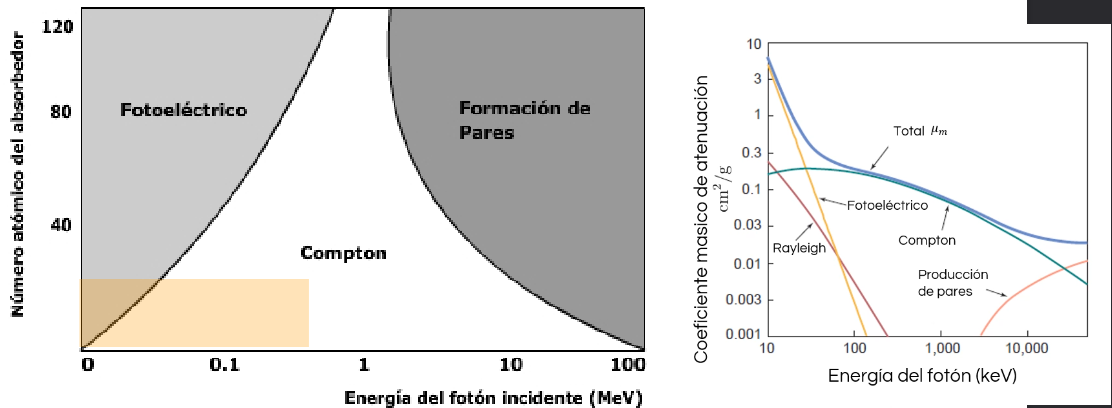
\includegraphics[width=0.7\textwidth]{figuras/p3.png}
  \caption{En la dispersión Rayleigh tenemos una pérdida de energía conforme hay un aumento en el coeficiente másico de atenuación, sin embargo, a diferencia del efecto fotoeléctrico (en ambos casos números de masa bajos) tiene una pendiente menos pronunciada que la de la dispersión Rayleigh.}
  \label{fig:p3}
\end{figure}














\item ¿Qué es la atenuación? ¿Cuál es la importancia del coeficiente lineal de atenuación en la imagenología biomédica? ¿Qué es la capa hemirreductora y para que se utiliza?


\begin{itemize}
  \item En general, la atenuación es una medida en que un haz de energía incidente puede penetrar algún material \citep{huda}. El coeficiente de atenuación lineal \ec{\mu } es la fracción de fotones incidentes removidos del haz incidente por unidad de longitud, por lo general este valor incrementa con el número atómico y en la radiología diagnóstica, éste decrece conforme aumenta la energía del fotón \citep{alpen,huda}. Para explicar la importancia de \ec{\mu}  en imagenología biomédica describimos a \ec{e^{-\mu x}} como la probabilidad de que un fotón atraviese un medio de grosor \ec{x} sin interacciones, esta probabilidad resulta en el producto en la probabilidad de que el fotón no interactúe por medio de los cinco procesos de interacción \citep{russ}:
  \ecc{e^{-\mu x}=\p{e^{-\omega  x}}\p{e^{-\tau  x}}\p{e^{-\sigma  x}}\p{e^{-\kappa  x}}\p{e^{-\pi  x}}=e^{-(\omega+\tau+\sigma+\kappa+\pi) x}}
  en donde \ec{\omega} es la interacción de dispersión coherente, \ec{\tau} es la absorción fotoeléctrica, \ec{\sigma} es la dispersión Compton, \ec{\kappa} es la producción de pares y  \ec{\pi} es la fotodesintegración. Esto nos muestra que los modos de interacción de los fotones con la materia resulta acumulativa, entonces, para un medio no homogéneo el coeficiente de atenuación lineal resulta en \ec{\mu=\Sigma_i \mu_i}, donde \ec{i} denota el número de componentes del medio, como ejemplo, en los sistema PET los detectores de anillo permiten obtener la distribución de intensidades con el coeficiente de atenuación lineal y construir imágenes aplicando métodos analíticos o iterativos.
  \item La capa hemirreductora es el grosor de un material que atenua un haz de fotones, normalmente de rayos X, a una exposición del \ec{50\%} usada para cuantificar haces polienergéticos (a diferencia del coeficiente de atenuación lineal que es para haces monoenergéticos), además, cuantifica la habilidad de un haz de fotones de penetrar tejido  \citep{russ}.
\end{itemize}













\item  Investigue ¿Qué es un filtrado de haz? ¿Por qué es importante que se haga un filtrado de haz?

El filtrado de haz consiste en absorber preferentemente fotones con energía específica, en imágenes de rayos X por ejemplo, la energía de los fotones filtrados es de baja energía. Su importancia radica en que cuando el haz de rayos X sale del tubo de rayos X contiene fotones de baja energía y estos tienen una probabilidad, aunque sea baja, de atravesar al paciente y contribuir al depósito de dosis y no a la imagen en sí. Como ejemplo, un filtro inherente es una capa de vidrio que detiene a los rayos X de baja energía y el filtro añadido es aquel en donde sí se puede seleccionar la energía de los fotones que se quiere filtrar \citep{alpen,russ}.











\item  Investigue ¿Qué es el endurecimiento de haz y como afecta a la calidad de imagen?


El endurecimiento del haz se refiere a la pérdida, selectiva, de fotones de menor energía de un haz policromático con filtro. Este efecto provoca que dé como resultado que haya un cambio en el espectro de rayos X, pero no de los picos de energía máximas, aunque sí lo hace la energía promedio que hace que aumente (lo cual puede que genere artefactos en la imagen), entonces, el concepto viene que el haz se vuelva más penetrante conforme aumente la energía promedio de los fotones \citep{edwin}.





\pagebreak



\item  Investigue el procedimiento para obtener una radiografía digital.


\begin{figure}[!ht]
  \center
  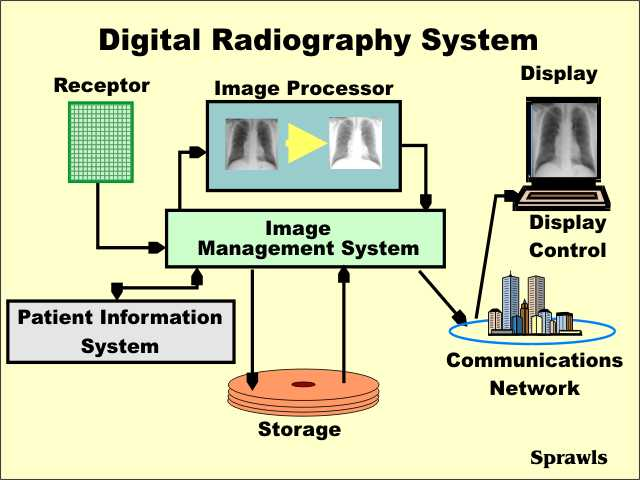
\includegraphics[width=0.4\textwidth]{figuras/p7.jpg}
  \caption{Procedimiento para obtener una radiografía digital. Figura recuperada de \url{http://www.sprawls.org/resources/DIGRAD/module.htm}.}
  \label{fig:p7}
\end{figure}

La detección digital consiste en transformar la energía de los fotones de rayos X (adquisición) en señales eléctricas (conversión analógica digital), la cual se presenta en imágenes digitales en escala de grises los cuales cuantifican cuánta radiación ha sido absorbida o atravesada por el paciente en la imagen digital








\item Investigue ¿Cuáles son las principales diferencias que existen entre la radiografía y la gammagrafía? Menciona por lo menos 3 y explique a detalle.














\end{enumerate}


\begin{multicols}{2}
\small{\bibliographystyle{apalike}
\bibliography{bib}}
\end{multicols}



%\ftikz{1.5}{figuras/fig.tikz}{}{fig:x}

\end{document}



